\section{Explotación}

Dado que ambos códigos hacen uso de una función considerada peligrosa, por lo que para poder compilarlo tendremos que proveerle a \textit{gcc} ciertas banderas:

\begin{quote}
\texttt{gcc -g -fno-stack-protector -z execstack nombreCodigo.c -o nombreCodigoCompilado -std=c99 -D\_FORTIFY\_SOURCE=0}
\end{quote}

\begin{center}
    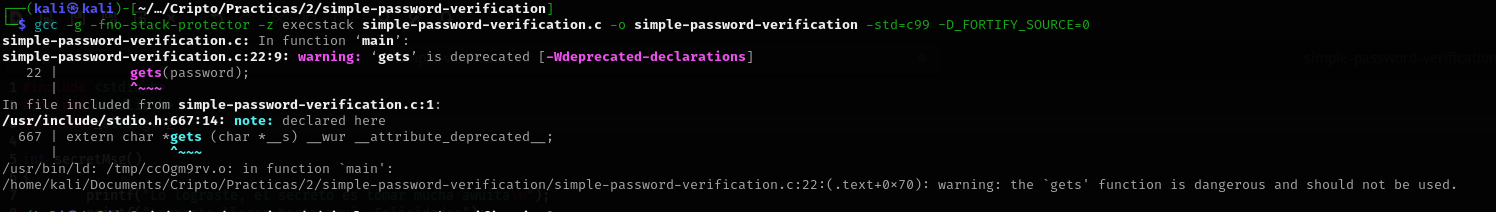
\includegraphics[scale=.3]{img/compilePassword.png}
\end{center}

\begin{center}
    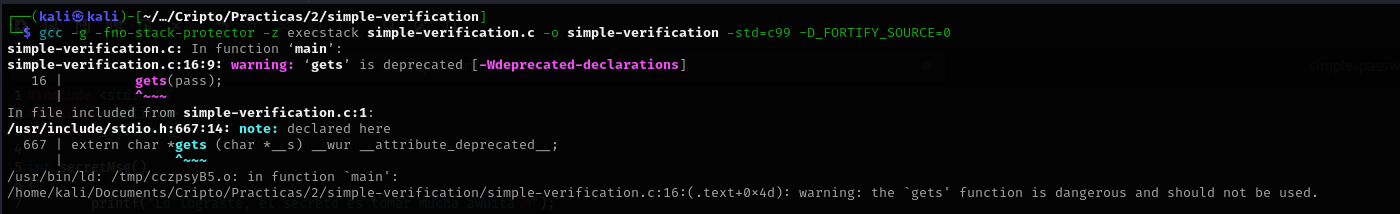
\includegraphics[scale=.3]{img/compileVerification.png}
\end{center}

Estas nos permiten indicarle al compilador lo siguiente:

\begin{itemize}
  \item \texttt{-g} Hace que el compilador incluya información de depuración que necesitaremos cuando usemos a GDB.
  \item \texttt{-fno-stack-protector} Hace que se desactive la protección del stack.
  \item \texttt{-z execstack} Hace que se pueda ejecutar código en el stack.
  \item \texttt{-std=c99} Establece el estándar C99.
  \item \texttt{-D\_FORTIFY\_SOURCE=0} Desactiva las optimizaciones de seguridad en las funciones de manejo de cadenas y buffers.
\end{itemize}

Una vez compilado el programa podemos ejecutarlo con GDB.

Lo ejecutamos de forma depurada con el comando \texttt{start}.

En el primer código, deseamos acceder a la función \texttt{granted()}, por lo que debemos de buscar su ubicación dentro del stack. Para ello podemos usar el siguiente comando de GDB \texttt{print granted}:

Hacemos lo mismo para el segundo código, donde el nombre de la función que buscamos es \texttt{secretMsg()}, ejecutando así en GDB \texttt{print secretMsg}:

\begin{center}
    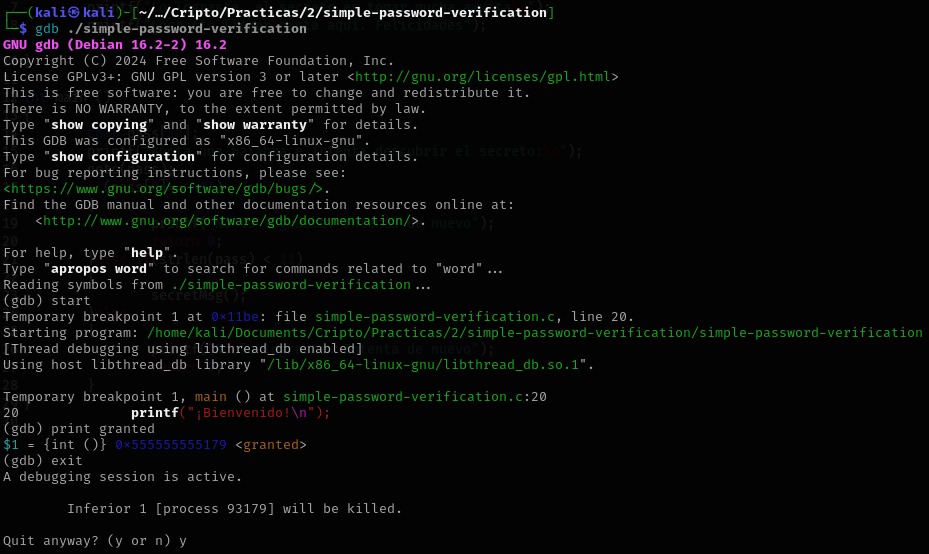
\includegraphics[scale=.5]{img/gdbPassword.png}
\end{center}

\begin{center}
    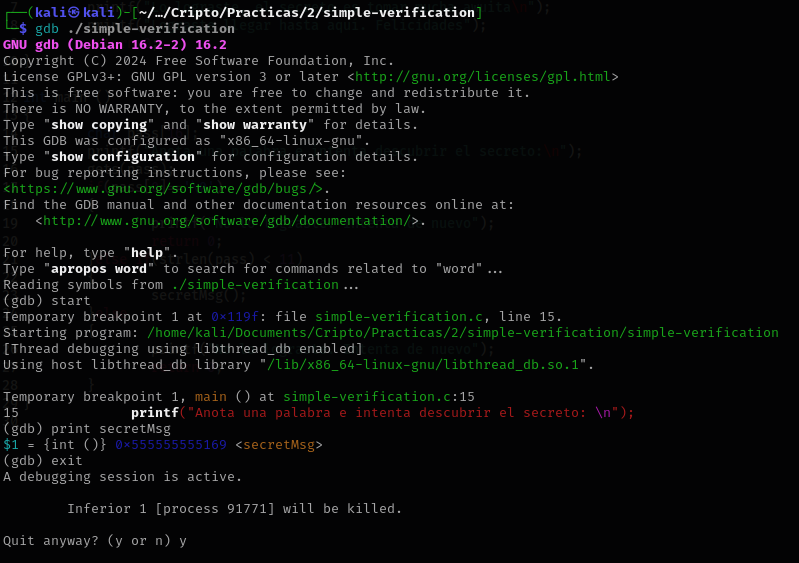
\includegraphics[scale=.5]{img/gdbVerification.png}
\end{center}

Anotamos las direcciones de ambas y salimos de GDB. El motivo de esto, es que, una vez que llenemos el buffer con su máxima capacidad, podamos escribir en el registro de dirección de retorno del stack, la dirección de memoria de dichas funciones.

De esta manera, nuestro exploit consistirá en una entrada de tipo string compuesta por una cantidad caracteres igual al límite del buffer concatenados con la dirección de memoria de ambas funciones. 

Una observación importante es que al momento de que la computadora lea la dirección de memoria, esta debe de estar en formato little endian, la cual consiste en dividir la dirección original en parejas de caracteres y añadirlos en una cadena en orden inverso, donde cada pareja le preceden los caracteres \texttt{\textbackslash x}.

Para realizar estos nos apoyaremos de python, de manera que nuestro exploit se ejecute bajo el siguiente comando:

\begin{quote}
\texttt{python3 -c 'print(''A''*\{límite del buffer\} + "[dirección de memoria de la función]") | ./[nombre del programa compilado]'}
\end{quote}


La bandera \texttt{-c} permite ejecutar python3 desde la línea de comandos. Hacemos que imprima una cantidad de caracteres igual al límite del buffer (en este caso usaremos a la letra A), y le concatenamos la dirección de la función en little endian. Dicha salida se la pasamos a nuestro programa para que la reciba como entrada al momento de ejecutarse.

Al momento de probar el exploit, intentamos con 16 A's (pues el es el tamaño de los dos arreglos que contienen nuestra entrada en los códigos), al no bastar les incrementamos uno hasta llegar al número 24.

De manera que para el primer código, el exploit quedó de la siguiente manera:

\begin{quote}
\texttt{python3 -c 'print(''A''*24 + "\textbackslash x79\textbackslash x51\textbackslash x55\textbackslash x55\textbackslash x55\textbackslash x55") | ./simple-password-verification'}
\end{quote}

\begin{center}
    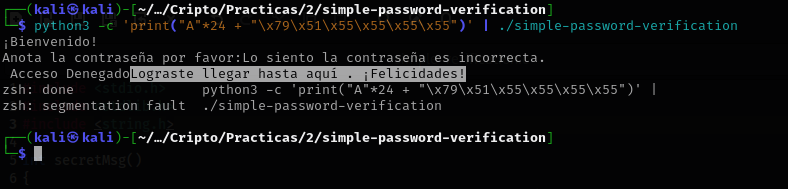
\includegraphics[scale=.5]{img/exploitPassword.png}
\end{center}

Mientras que para el segundo código, quedó así:

\begin{quote}
\texttt{python3 -c 'print(''A''*24 + "\textbackslash x69\textbackslash x51\textbackslash x55\textbackslash x55\textbackslash x55\textbackslash x55") | ./simple-verification'}
\end{quote}

\begin{center}
    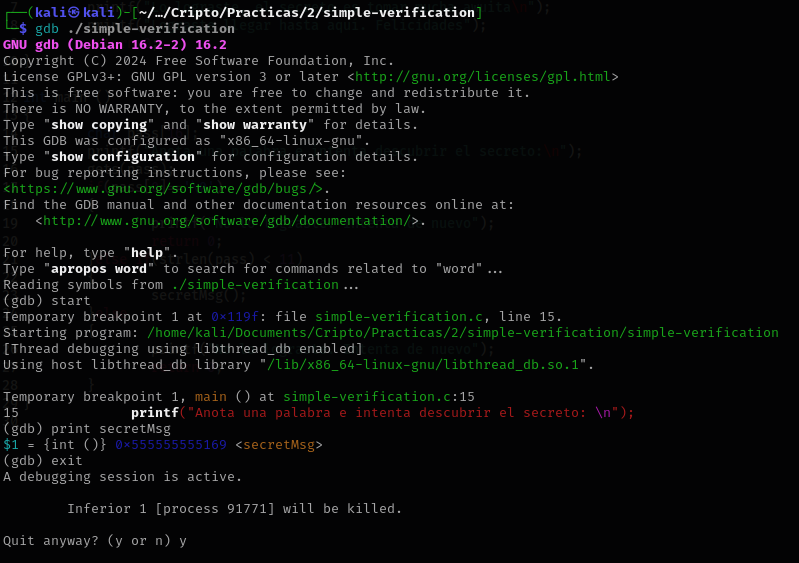
\includegraphics[scale=.5]{img/gdbVerification.png}
\end{center}

Podemos ver que en ambos casos, se pudo acceder a la función adecuada, pues recibimos los mensajes de aceptación.